\pagestyle{plain}
\appendix
\chapter{Trimming DAC configuration examples}\label{DacAppendix}
\section{Writing commands}
\begin{figure}[H]
	\centering
	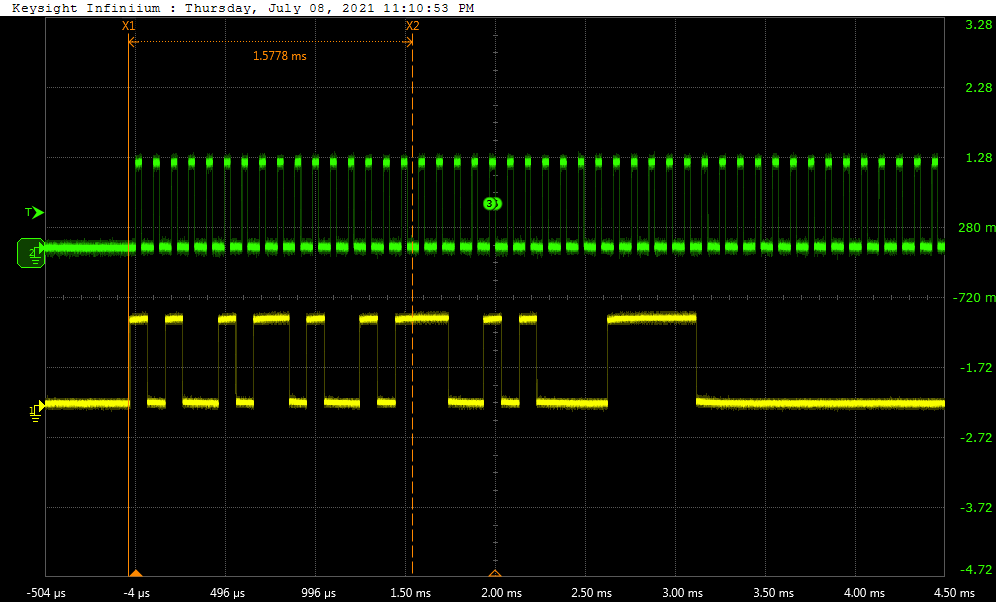
\includegraphics[width=0.6\linewidth]{IMG/ch5/probe/09-08-2021_ch05-write31-baselinedac1}
	\caption{Writing sequence, channel 5, word 31, DAC 1\\{\color{magenta}purple}= clock, {\color{blue}blue}= data out}
	\label{fig:ch05write31}
\end{figure}

\begin{figure}[H]
	\centering
	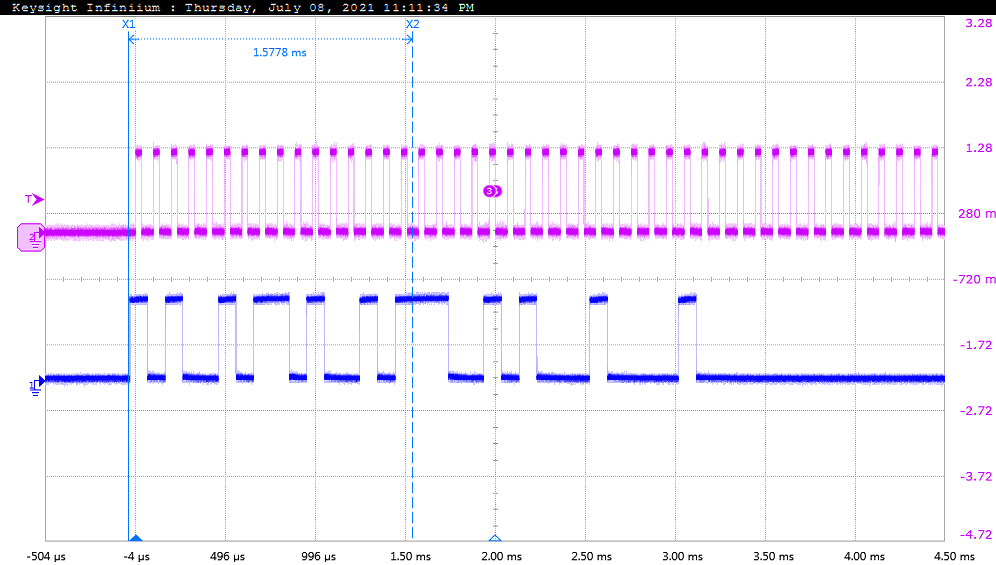
\includegraphics[width=0.6\linewidth]{IMG/ch5/probe/09-08-2021_ch05-write33-baselinedac1}
	\caption{Writing sequence, channel 5, word 33, DAC 1\\{\color{magenta}purple}= clock, {\color{blue}blue}= data out}
	\label{fig:ch05write33}
\end{figure}
%\newpage
%\thispagestyle{plain}
\begin{figure}[H]
	\centering
	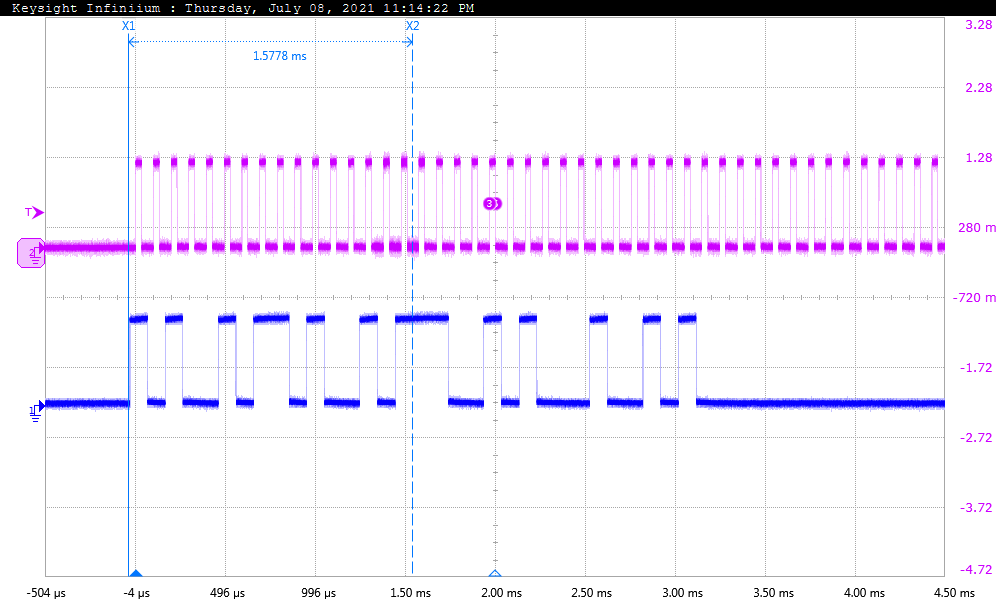
\includegraphics[width=0.6\linewidth]{IMG/ch5/probe/09-08-2021_ch05-write37-baselinedac1}
	\caption{Writing sequence, channel 5, word 37, DAC 1\\{\color{magenta}purple}= clock, {\color{blue}blue}= data out}
	\label{fig:ch05write37}
\end{figure}

\begin{figure}[H]
	\centering
	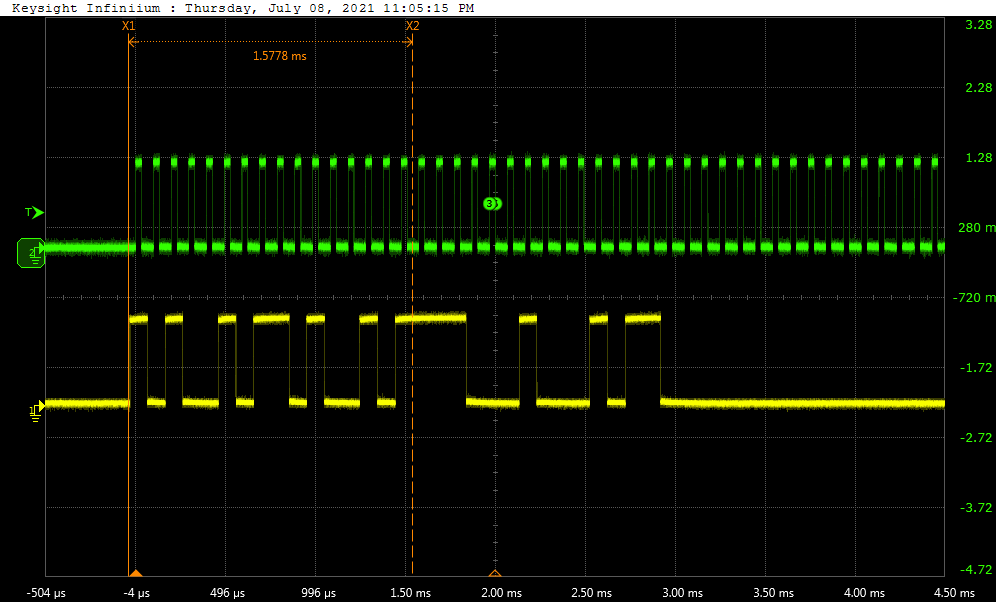
\includegraphics[width=0.6\linewidth]{IMG/ch5/probe/09-08-2021_ch17-write44-baselinedac1}
	\caption{Writing sequence, channel 17, word 44, DAC 1\\{\color{magenta}purple}= clock, {\color{blue}blue}= data out}
	\label{fig:ch17write44}
\end{figure}
\section{Reading commands}
\begin{figure}[H]
	\centering
	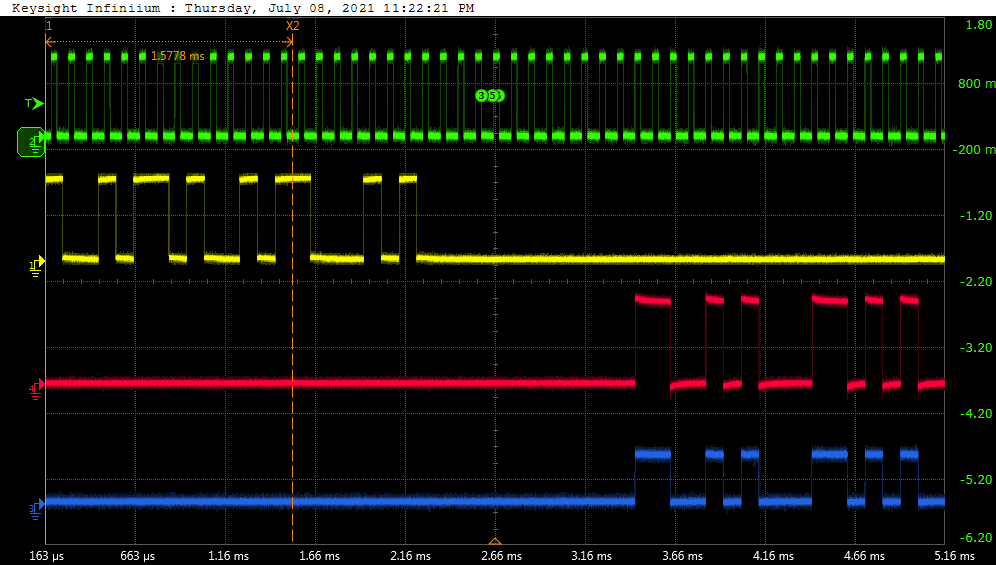
\includegraphics[width=0.6\linewidth]{IMG/ch5/probe/09-08-2021_ch05-read53-baselinedac1}
	\caption{Reading sequence, channel 5, word 53, DAC 1\\{\color{magenta}purple}= clock, {\color{blue}blue}= data out,\\{\color{cyan}cyan}= data in, {\color{orange}orange}= data from chip}
	\label{fig:ch05write53}
\end{figure}
%\newpage
%\thispagestyle{plain}
\begin{figure}[H]
	\centering
	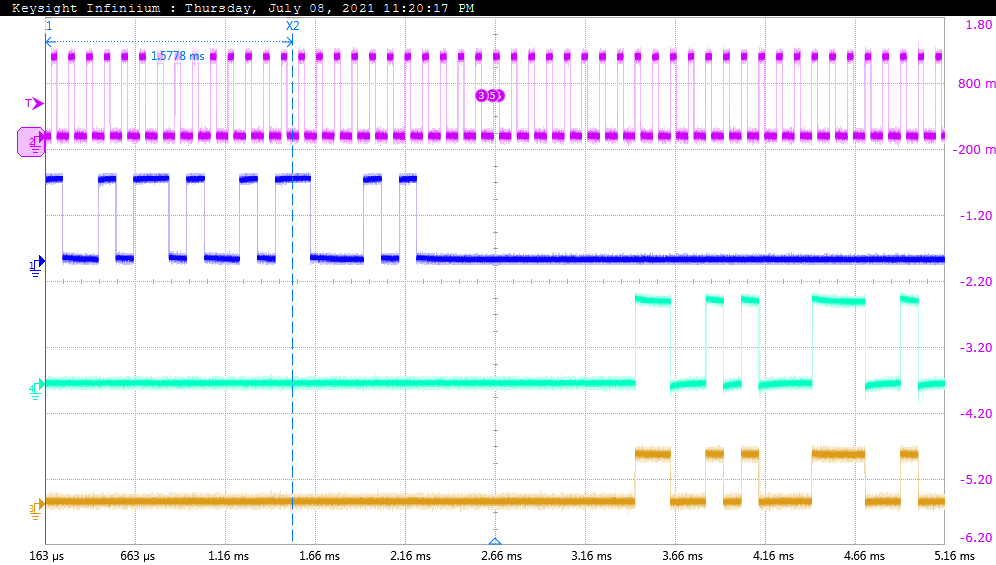
\includegraphics[width=0.6\linewidth]{IMG/ch5/probe/09-08-2021_ch05-read57-baselinedac1}
	\caption{Reading sequence, channel 5, word 57, DAC 1\\{\color{magenta}purple}= clock, {\color{blue}blue}= data out,\\{\color{cyan}cyan}= data in, {\color{orange}orange}= data from chip}
	\label{fig:ch05write57}
\end{figure}

\begin{figure}[H]
	\centering
	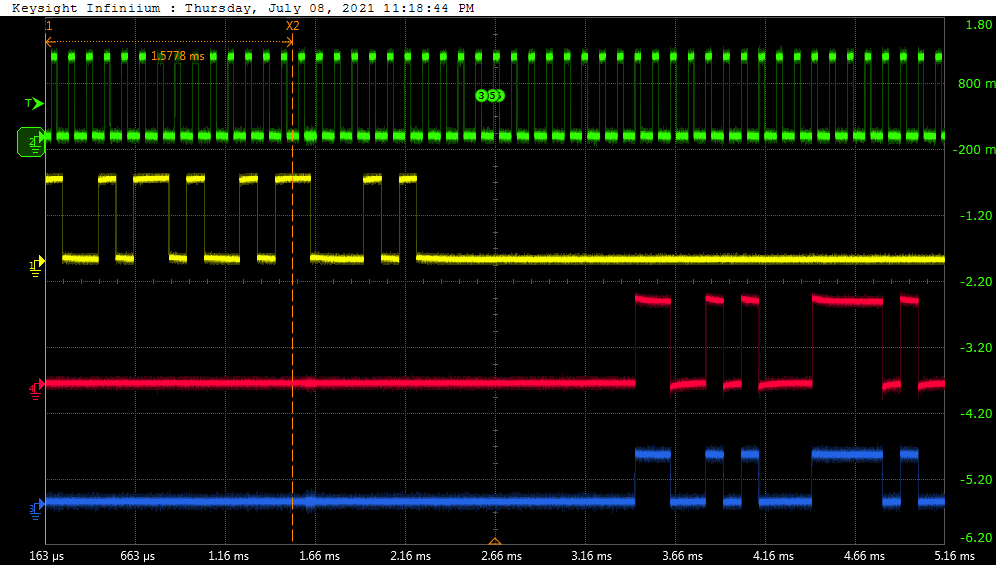
\includegraphics[width=0.6\linewidth]{IMG/ch5/probe/09-08-2021_ch05-read61-baselinedac1}
	\caption{Reading sequence, channel 5, word 61, DAC 1\\{\color{magenta}purple}= clock, {\color{blue}blue}= data out,\\{\color{cyan}cyan}= data in, {\color{orange}orange}= data from chip}
	\label{fig:ch05write61}
\end{figure}

\begin{figure}[H]
	\centering
	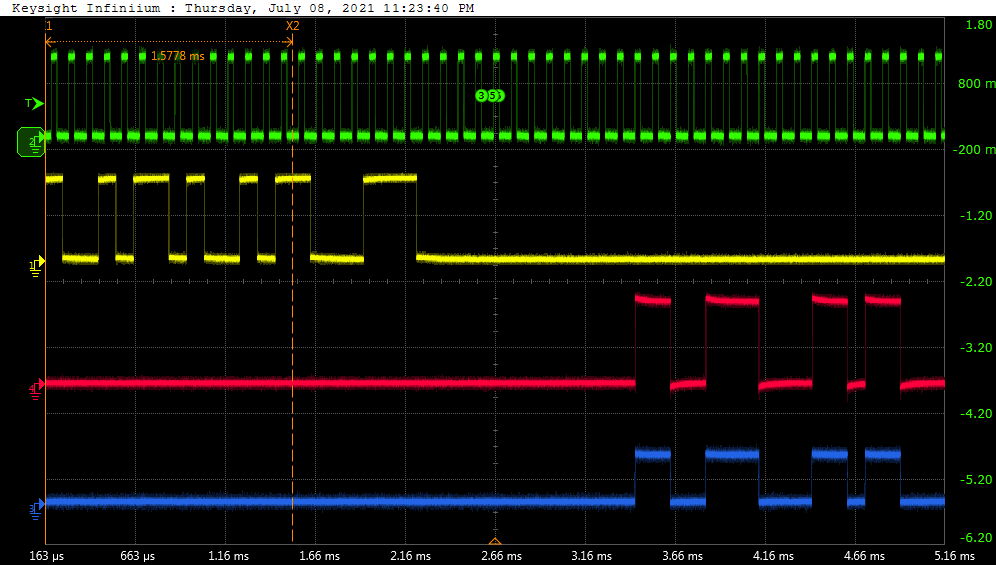
\includegraphics[width=0.6\linewidth]{IMG/ch5/probe/09-08-2021_ch07-read54-baselinedac1}
	\caption{Reading sequence, channel 7, word 54, DAC 1\\{\color{magenta}purple}= clock, {\color{blue}blue}= data out,\\{\color{cyan}cyan}= data in, {\color{orange}orange}= data from chip}
	\label{fig:ch07write54}
\end{figure}